\documentclass[a4paper,kulak]{kulakarticle} %options: kul or kulak (default)

\usepackage[utf8]{inputenc}
\usepackage[dutch]{babel}
\usepackage{mhchem}
\usepackage{caption}
\usepackage{subcaption}



\date{Academiejaar 2018 -- 2019}
\address{
  Master of Physics \\
  Visits to Research Laboratories in Belgium.  \\
  Prof. T. Cocolius}
\title{Visit of the Magnetometry Laboratory
	Report} 
\author{Jérôme Neirynck\\ Frederik Van Eecke\\ Robin Vrielynck\\ Robin Brambilla}

\begin{document}

\maketitle


\section{The cesium magnetometer.}
In order to make dipole measurements of the neutron possible a high resolution magnetic field sensor is necessary to fulfill the magnetic field stability requirement. The Cesium magnetometer used is based on the concept of optically detected magnetic resonance (ODMR) spectroscopy. Cesium is an alkali metal, which means there is one valence electron in an s-orbital. More specific the electronic configuration of cesium can be described as $[Xe]6s^{1}$.Therefore the interaction of Cesium with an external magnetic field is governed by the magnetic moment of its unpaired electron, aligned with the electron spin. Since the absorption of resonant polarized light also depends on the electron spin it is possible to link magnetic interactions via light dependent properties.\\ 

The first step in understanding ODMR is a better understanding of the hyperfine and Zeeman structure in cesium. The only stable isotope of cesium is $\ce{^{133}_{55}Cs}$, which is used in all applications. It has a nuclear spin of $\frac{7}{2}.$ The interaction of this nuclear spin with the $J=\frac{1}{2}$ angular momentum provided by the valence electron results in a splitting of the ground state $6S_{\frac{1}{2}}$ into two hyperfine states $F = |I \pm J|$. These two hyperfine states are separated by an energy difference corresponding to a frequency of $9.2 GHz$. An energy scheme of $Cs$ is shown in figure \ref{fig:hyperfine}. The transition $D_{1}$ to the first excited state lies in the near-infrared (894.6 nm). The hyperfine interaction also splits this first excited state $6P_{\frac{1}{2}}$ into two hyperfine states corresponding with $f = 3,4$ separated by an energy difference corresponding to $1.2 GHz$. The zeeman splitting observed when an magnetic field is observed causes a further splitting of the hyperfine states into $2F+1$ degenerate sublevels, as shown in figure \ref{fig:zeeman}.

\begin{figure}[h!]
	\centering
	\begin{subfigure}[L]{.5\textwidth}
		\centering
		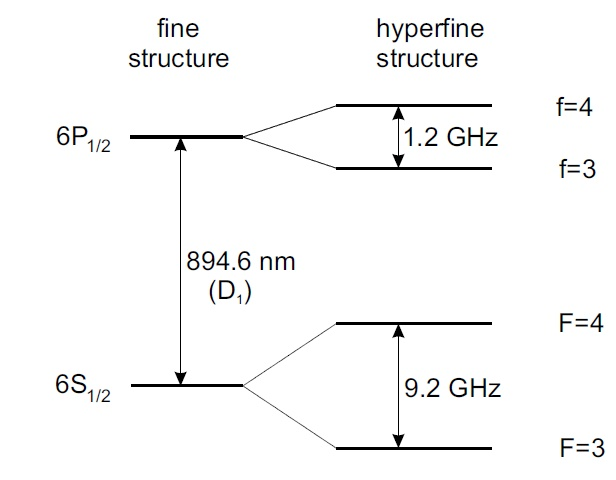
\includegraphics[width=.7\linewidth]{hyperfine}
		\caption{Energy scheme of $\ce{^{133}Cs}$. $D_{1}$ transition with hyperfine structure.}
		\label{fig:hyperfine}
	\end{subfigure}%
	\begin{subfigure}[R]{.5\textwidth}
		\centering
		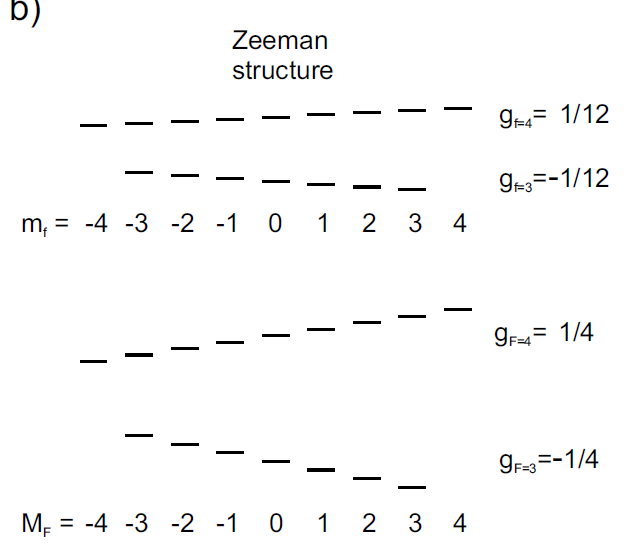
\includegraphics[width=.7\linewidth]{zeeman}
		\caption{Linear Zeeman effect in a small magnetic field (not to scale). The Zeeman levels presented are sublevels of the hyperfine levels presented in \ref{fig:hyperfine} }
		\label{fig:zeeman}
	\end{subfigure}
\end{figure}


\begin{thebibliography}{plain}
	\bibitem{} Laser-pumped cesium magnetometers for the
	PSI-nEDM experiment,Stephan Gröger,2005,München.
	
	\bibitem{}
\end{thebibliography}



\end{document}